\documentclass[11pt,a4paper]{article}

% ---------- packages ----------
\usepackage[T1]{fontenc}
\usepackage[utf8]{inputenc}
\usepackage[margin=2.4cm,top=2.6cm,bottom=2.6cm]{geometry}
\usepackage{newtxtext,newtxmath}
\usepackage[scaled=0.86]{inconsolata}
\usepackage{microtype}
\usepackage{booktabs}
\usepackage{tabularx}
\usepackage{array}
\usepackage{multirow}
\usepackage{xcolor}
\usepackage{tikz}
\usepackage{pgfplots}
\usepackage{amsmath}
\usepackage{enumitem}
\usepackage{titlesec}
\usepackage{caption}
\usepackage{listings}
\usepackage{fancyhdr}
\usepackage{underscore}
\usepackage[colorlinks=true,linkcolor=accent,urlcolor=accent,citecolor=accent]{hyperref}

\usetikzlibrary{positioning,arrows.meta,calc,fit,backgrounds,shapes.geometric,decorations.pathreplacing}
\pgfplotsset{compat=1.18}

% ---------- palette ----------
\definecolor{accent}{HTML}{1F6F6B}   % verdigris
\definecolor{rust}{HTML}{A8442A}     % rust
\definecolor{ink}{HTML}{1A1D1E}
\definecolor{mute}{HTML}{5E6A6B}
\definecolor{pale}{HTML}{E8F0EF}
\definecolor{palerust}{HTML}{F6E7E1}
\definecolor{rule}{HTML}{C8D4D3}

% ---------- section styling ----------
\titleformat{\section}{\normalfont\large\bfseries\color{accent}}{\thesection}{0.7em}{}
\titleformat{\subsection}{\normalfont\normalsize\bfseries\color{ink}}{\thesubsection}{0.6em}{}
\titlespacing*{\section}{0pt}{1.6em plus .3em minus .2em}{0.6em}
\captionsetup{font=small,labelfont={bf,color=accent},width=.94\textwidth}

\pagestyle{fancy}\fancyhf{}
\renewcommand{\headrulewidth}{0.4pt}
\fancyhead[L]{\small\color{mute}eACBN0 in \texttt{hp.x}}
\fancyhead[R]{\small\color{mute}\thepage}

\lstset{
  basicstyle=\ttfamily\scriptsize,
  breaklines=true, columns=fullflexible, keepspaces=true,
  backgroundcolor=\color{pale!60}, frame=leftline, framerule=1.2pt,
  rulecolor=\color{accent}, xleftmargin=8pt, framexleftmargin=8pt,
  aboveskip=8pt, belowskip=8pt,
  commentstyle=\color{mute}\itshape,
  keywordstyle=\color{accent}\bfseries,
}

\newcommand{\C}[1]{\texttt{\small #1}}
\newcommand{\good}{\textcolor{accent}{\textbf{\checkmark}}}

% ================================================================
\begin{document}

\begin{center}
{\LARGE\bfseries eACBN0 in \texttt{hp.x}}\\[3pt]
{\large\color{mute} Transplanting the DFT+U+V Hubbard-parameter kernels\\
from a QE 7.3 fork's \texttt{pw.x} into \texttt{hp.x}}\\[10pt]
{\small Validation report \quad\textbullet\quad 4 September 2026}
\end{center}

\vspace{4pt}
\noindent\textcolor{rule}{\rule{\textwidth}{0.8pt}}
\vspace{6pt}

\noindent
\textbf{Goal.} One binary that produces both the pseudo-hybrid (ACBN0) and the
linear-response (DFPT) estimate of $U$ from a \emph{single} ground state.

\smallskip
\noindent
\textbf{Method reference.} S. Lee and Y.-W. Son, \emph{Phys.\ Rev.\ Research}
\textbf{2}, 043410 (2020), named in \C{example/Howto2.pdf}. ACBN0 itself:
Agapito, Curtarolo and Buongiorno Nardelli, \emph{Phys.\ Rev.\ X} \textbf{5},
011006 (2015).

\smallskip
\noindent
\textbf{Deliverable.} \C{HP/src/eACBN0.f90} --- 4234 lines, two modules,
22 subroutines and one function --- plus seven modified files in \C{HP/src/}.

\vspace{2pt}
\noindent\textcolor{rule}{\rule{\textwidth}{0.8pt}}

% ================================================================
\section{Headline}

Both branches now run on an ordinary DFT+U ground state, and both reproduce the
original authors' own MnO reference output \textbf{exactly}: every $U$, every
$V$, every cell vector --- 28 blocks, 168 lines, empty diff.

\begin{table}[h]
\centering\small
\begin{tabular}{lrrr}
\toprule
Quantity & Reference & our \C{pw.x} & our \C{hp.x} \\
\midrule
Mn$_A$ 3d on-site, \C{V[1,1]} cell \C{[0 0 0]} & 5.2344 & \textbf{5.2344} & \textbf{5.2344} \\
Mn$_B$ 3d on-site, \C{V[2,2]}                  & 5.2344 & \textbf{5.2344} & \textbf{5.2344} \\
O 2p on-site, \C{V[3,3]}, \C{V[4,4]}           & 3.4161 & \textbf{3.4161} & \textbf{3.4161} \\
Mn--O inter-site, cell \C{[-1 -1 0]}           & 2.9031 & \textbf{2.9031} & \textbf{2.9031} \\
Mn--O inter-site, cells \C{[-1 0 -1]}, \C{[-1 0 0]} & 2.9042 & \textbf{2.9042} & \textbf{2.9042} \\
\midrule
absolute magnetisation ($\mu_B$/cell)          & 9.36   & 9.36 & --- \\
\bottomrule
\end{tabular}
\caption{All values in eV. Source: \C{example/MnO.acbn0.out}, QE v7.3, 128
processors, 5 January 2024, \C{acbn0_type = 2}. Our \C{hp.x} column is
\C{MnO_ref_v3/hp.out}, produced on \C{ldaU} bookkeeping (stage V3).}
\end{table}

\noindent
Four latent bugs were found and fixed; two of them would have returned a
plausible wrong number rather than crashing (\S\ref{sec:bugs}). One capability
was deliberately traded away (\S\ref{sec:open}).

\smallskip
\noindent
\textbf{Final regression:} 15 passed, 0 failed, on a single binary.

% ================================================================
\section{Why \texttt{hp.x} could not do this already}

The fork's patch (\C{qe-7.3_ehub_uv.diff}) touches 60 files. \textbf{None of them
is under \C{HP/}} --- the authors implemented DFT+U+V in \C{pw.x} only. That single
fact is the root cause of every bug in \S\ref{sec:bugs}.

\C{pw.x} initialises \C{MODULE ldaV} from \emph{two} paths, and \C{hp.x} only ever
walks the second:

\begin{center}
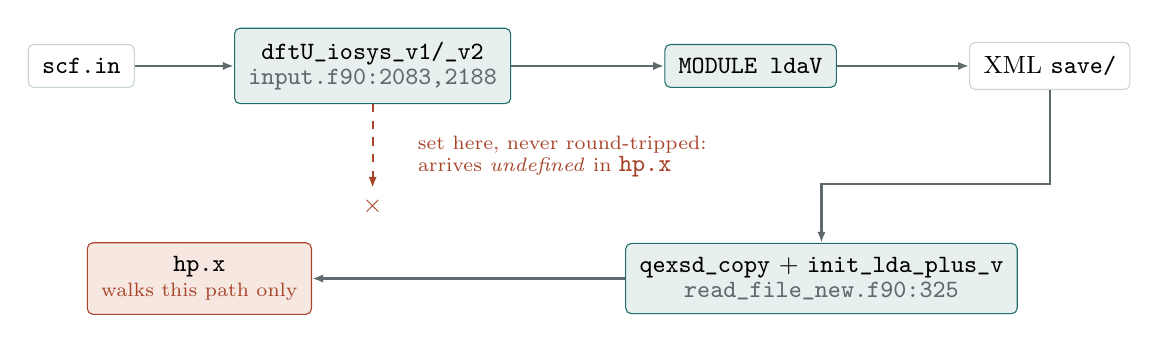
\begin{tikzpicture}[
  font=\small,
  box/.style={draw=rule,fill=white,rounded corners=2pt,inner sep=5pt,align=center},
  gbox/.style={box,fill=pale,draw=accent},
  rbox/.style={box,fill=palerust,draw=rust},
  ar/.style={-{Latex[length=4pt]},draw=mute,thick},
]
\node[box]  (scf)   at (0,0)      {\C{scf.in}};
\node[gbox] (iosys) at (3.7,0)    {\C{dftU_iosys_v1/_v2}\\[-2pt]{\scriptsize\color{mute}\C{input.f90:2083,2188}}};
\node[gbox] (ldav)  at (8.5,0)    {\C{MODULE ldaV}};
\node[box]  (xml)   at (12.3,0)   {XML \C{save/}};
\node[gbox] (qexsd) at (9.4,-2.7) {\C{qexsd_copy} + \C{init_lda_plus_v}\\[-2pt]{\scriptsize\color{mute}\C{read_file_new.f90:325}}};
\node[rbox] (hp)    at (1.5,-2.7) {\C{hp.x}\\[-2pt]{\scriptsize\color{rust}walks this path only}};

\draw[ar] (scf)   -- (iosys);
\draw[ar] (iosys) -- (ldav);
\draw[ar] (ldav)  -- (xml);
\draw[ar] (xml.south) -- (12.3,-1.5) -- (9.4,-1.5) -- (qexsd.north);
\draw[ar] (qexsd) -- (hp);

\draw[dashed,rust,thick,-{Latex[length=4pt]}] (iosys.south) -- (3.7,-1.55);
\node[rust]                       at (3.7,-1.78) {$\times$};
\node[rust,font=\scriptsize,align=left,anchor=west] at (4.15,-1.15)
      {set here, never round-tripped:\\ arrives \emph{undefined} in \C{hp.x}};
\end{tikzpicture}
\end{center}

\noindent
Anything set only on the input path therefore arrives \emph{undefined} in
\C{hp.x}. Rather than hunt for these one at a time, all 35 \C{ldaV} module
variables were swept against two questions --- does it have an initialiser, and
is it assigned in a file \C{hp.x}'s read path executes? --- which turned an
open-ended search into a closed list.

% ================================================================
\section{Method: one variable per rung}

The dangerous failure mode here is not a crash but a plausible wrong number, so
no stage changes two things at once. Ten rungs, each moving exactly one of
\{driver, kernel, bookkeeping, ground state\}:

\begin{center}
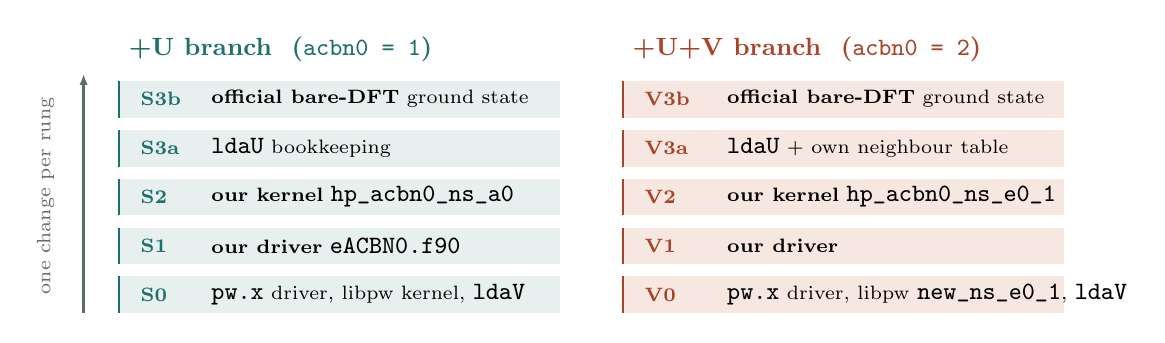
\begin{tikzpicture}[font=\scriptsize, xscale=1.0, yscale=0.62]
  \definecolor{s1}{HTML}{1F6F6B}
  \foreach \i/\lab/\note in {
     0/S0/{\C{pw.x} driver, libpw kernel, \C{ldaV}},
     1/S1/{\textbf{our driver} \C{eACBN0.f90}},
     2/S2/{\textbf{our kernel} \C{hp_acbn0_ns_a0}},
     3/S3a/{\textbf{\C{ldaU}} bookkeeping},
     4/S3b/{\textbf{official bare-DFT} ground state}} {
     \fill[pale] (0,\i) rectangle (5.6,{\i+0.75});
     \draw[accent,line width=1pt] (0,\i) -- (0,{\i+0.75});
     \node[anchor=west,accent] at (0.15,{\i+0.38}) {\bfseries \lab};
     \node[anchor=west] at (1.05,{\i+0.38}) {\note};
  }
  \foreach \i/\lab/\note in {
     0/V0/{\C{pw.x} driver, libpw \C{new_ns_e0_1}, \C{ldaV}},
     1/V1/{\textbf{our driver}},
     2/V2/{\textbf{our kernel} \C{hp_acbn0_ns_e0_1}},
     3/V3a/{\textbf{\C{ldaU}} + own neighbour table},
     4/V3b/{\textbf{official bare-DFT} ground state}} {
     \fill[palerust] (6.4,\i) rectangle (12.0,{\i+0.75});
     \draw[rust,line width=1pt] (6.4,\i) -- (6.4,{\i+0.75});
     \node[anchor=west,rust] at (6.55,{\i+0.38}) {\bfseries \lab};
     \node[anchor=west] at (7.6,{\i+0.38}) {\note};
  }
  \node[accent,anchor=west,font=\small\bfseries] at (0,5.4) {+U branch \ (\C{acbn0 = 1})};
  \node[rust,anchor=west,font=\small\bfseries]   at (6.4,5.4) {+U+V branch \ (\C{acbn0 = 2})};
  \draw[-{Latex[length=4pt]},mute,thick] (-0.45,0) -- (-0.45,4.9);
  \node[mute,rotate=90,anchor=south] at (-0.7,2.4) {one change per rung};
\end{tikzpicture}
\end{center}

\begin{table}[h]
\centering\small
\setlength{\tabcolsep}{4.5pt}
\begin{tabular}{llllll}
\toprule
Stage & Driver & Kernel & Bookkeeping & Ground state & Result (eV) \\
\midrule
S0  & \C{pw.x sum_band} & libpw \C{new_ns_a0} & \C{ldaV} & ACBN0-converged & 9.2501 / 9.2509 / 4.2471 \\
S1  & \emph{\C{eACBN0.f90}} & libpw \C{new_ns_a0} & \C{ldaV} & same & identical \\
S2  & \C{eACBN0.f90} & \emph{\C{hp_acbn0_ns_a0}} & \C{ldaV} & same & byte-identical \\
S3a & \C{eACBN0.f90} & our kernel & \emph{\C{ldaU}} & same & identical \\
S3b & \C{eACBN0.f90} & our kernel & \C{ldaU} & \emph{official bare-DFT} & 10.5455 / 4.2717 \\
\midrule
V0  & \C{pw.x sum_band} & libpw \C{new_ns_e0_1} & \C{ldaV} & eACBN0-converged & 7.7065 / 2.6538 $+\,V$ \\
V1  & \emph{\C{eACBN0.f90}} & libpw \C{new_ns_e0_1} & \C{ldaV} & same & identical, 456 lines \\
V2  & \C{eACBN0.f90} & \emph{\C{hp_acbn0_ns_e0_1}} & \C{ldaV} & same & identical, 456 lines \\
V3a & \C{eACBN0.f90} & our kernel & \emph{\C{ldaU}} & same & identical, 456 lines \\
V3b & \C{eACBN0.f90} & our kernel & \C{ldaU} & \emph{official bare-DFT} & 10.5455 / 4.2717 $+\,V$ \\
V4  & \C{eACBN0.f90} & our kernel & \C{ldaU} \emph{+ background} & any & \emph{multi-channel}, 204 lines \\
\bottomrule
\end{tabular}
\caption{\emph{Italic} marks the one thing that changed on that rung.}
\end{table}

\subsection{S3b needed its own reference}

S3b changes the input \emph{data}, not the code, so its number legitimately
moves and cannot be checked by a diff against S3a. Getting \C{pw.x} to evaluate
ACBN0 on an official ground state was blocked at first: with \C{lda_plus_v} set,
\C{read_scf} reads \C{occupation_uv.txt} unconditionally
(\C{io_rho_xml.f90:644}) and an official save has only the \C{ldaU}
\C{occup.txt}. Solved in two steps --- step~1 with \C{lacbn0 = .false.} (so
$U^{\text{ehub}} = V^{\text{ehub}} = 0$ and the Hamiltonian is the official one)
writes the file; step~2 does one ACBN0 evaluation on it.

\begin{center}\small
\begin{tabular}{lrrl}
\toprule
& \C{pw.x} one-shot & \C{hp.x} S3b & \\
\midrule
Ni1 3d & 10.5455 & 10.5455 & exact \\
Ni2 3d & 10.5455 & 10.5455 & exact \\
O \ 2p &  4.2718 &  4.2717 & last printed digit \\
$\mathrm{Tr}[n_s]$ atom 1 & 8.46278 & 8.4628 & exact \\
\midrule
\multicolumn{4}{l}{\footnotesize control: step-1 $E_{\rm tot}$ = official \C{../NiO} $E_{\rm tot}$ = $-737.16322501$ Ry}\\
\bottomrule
\end{tabular}
\end{center}

% ================================================================
\section{Static faithfulness of the transplant}

A numerical match on three systems is strong evidence, but not proof that the
kernels were copied faithfully rather than made to agree. So the transplanted
routines were also diffed against \C{PW/src/new_ns_v.f90} \emph{statically}, by
a script that

\begin{enumerate}[leftmargin=1.4em,itemsep=1pt]
\item joins Fortran continuation lines into whole statements and strips
      comments and blanks,
\item splits each routine at its first executable statement, keeping only the
      body (the preamble necessarily changes: \C{USE ldaV} becomes
      \C{USE ldaU}),
\item collapses every mechanical rename to a common token
      (\C{wfcv}$\leftrightarrow$\C{wfcU}, \C{ofstv}$\leftrightarrow$\C{offsetU},
      \C{ehub_nn_vect}$\leftrightarrow$\C{nn_vect}, and 24 more), and
\item canonicalises the \emph{intended} systematic edits: the clock labels,
      the dropped SCF mixing, and the dropped \C{remove_ehub_u/v} masks.
      Note what is \emph{not} canonicalised any more --- before stage V4 this
      step also had to collapse \C{ehub_l(m,nt)} to a scalar, which hid every
      $m$ index from the comparison. It no longer does.
\end{enumerate}

\noindent
Whatever survives is a genuine difference. The result:

\begin{table}[h]
\centering\small
\begin{tabular}{llrrl}
\toprule
Our routine & From & Stmts & Diff & Nature of the difference \\
\midrule
\C{hp_acbn0_ns_a0}    & \C{new_ns_a0} 233--635        & 176 & 0 & --- \\
\C{hp_acbn0_orberi}   & \C{orberi} 3780--3819         &  25 & 6 & dummy arg renamed \C{lp1} \\
\C{hp_acbn0_ns_e0_1}  & \C{new_ns_e0_1} 636--1808     & 577 & 8 & \C{stop_acbn0} short-circuit dropped \\
\C{hp_acbn0_ns_v}     & \C{new_ns_v} 10--232          & 103 & 0 & --- \\
\C{hp_acbn0_symm_n4}  & \C{symmetrize_n4} 2964--3167  &  86 & 1 & bug 4 guard \\
\C{hp_acbn0_symm_n4m} & \C{symmetrize_n4m} 3168--3399 & 104 & 1 & bug 4 guard \\
\C{hp_acbn0_symm_n5}  & \C{symmetrize_n5} 3400--3779  & 174 & 2 & bug 4 + bug 3 guards \\
\midrule
\textbf{total} & & \textbf{1245} & \textbf{18} & 3 distinct classes \\
\bottomrule
\end{tabular}
\caption{1245 canonicalised executable statements; 18 differing statements, in
3 classes, every one deliberate. Measured \emph{after} stage V4, where the
$m$ index is no longer collapsed --- so \C{ehub_l(m1,nt)} must now match
\C{lch(m1,nt)} literally, index by index. Two kernels come out at zero. The
script is \C{normdiff4.py} and is re-runnable.}
\end{table}

\noindent
This is a strictly stronger test than the one stage V3 could support. There,
the $m$ index had to be canonicalised away on both sides, so an incorrectly
restored index would have gone unnoticed; here all 225 restored indices must
agree with the fork literally, and they do. The \C{remove_ehub_*} masks are
still omitted rather than set to 1 --- equivalent whenever the \C{pw.x} run
used the documented default, and precisely why a run that masks a channel
cannot yet be reproduced (\S\ref{sec:open}).

% ================================================================
\section{Four latent bugs}\label{sec:bugs}

\subsection*{Bug 1 --- \texttt{remove_ehub_u} / \texttt{remove_ehub_v} undefined \ \textcolor{mute}{(silent)}}

No initialiser in \C{ldaV.f90}; assigned only at \C{input.f90:2083}. The kernels
multiply the final $U$ by them \emph{twice}. Undefined, this does not crash ---
it silently scales or zeroes every Hubbard parameter. Not hypothetical:
\C{example/GaAs.acbn0.in_noncollienar} sets \C{remove_ehub_u(1,1) = 0} to kill
the $s$-channel $U$.

\subsection*{Bug 2 --- \texttt{iunwfc} is closed at the insertion point \ \textcolor{rust}{(crash)}}

\C{read_file} buffers the wavefunctions to \C{iunwfc} and then closes it with
\C{close_buffer(..., 'KEEP')} (\C{read_file_new.f90:62}). \C{'KEEP'} preserves
the \emph{files}, but the call also deregisters the unit, so \C{get_buffer}
falls through to \C{davcio} on a closed unit. Official \C{hp.x} never trips this
because DFPT reads through \C{iuwfc}, which is opened later in \C{hp_openfil_q}.

\subsection*{Bug 3 --- \texttt{hubbard_get_nnc} returns an undefined index \ \textcolor{rust}{(crash, or worse)}}

\C{PW/src/hubbard_nns.f90:241}. \C{nnc} is assigned only inside
\C{IF (MAXVAL(ehub_nn_vect(...)) == 1)}, so a cell carrying no neighbour pair
falls through untouched. \C{hubbard_symmetry} then asks for the index of a
\emph{rotated} cell --- which is not guaranteed to be one of the occupied ones
--- and \C{symmetrize_n5} indexes \C{n(nnc)} with whatever was on the stack.

It never fires on the fork's own NiO ground state; it fires on the official one,
with an \emph{identical} neighbour table, identical symmetry (12 operations)
and identical manifold. In an optimised build a garbage index is silent
whenever it happens to land in a mapped page. The optimised build gave only a
UCX backtrace; a rebuild with \C{-check bounds,uninit -fpe0} named it at once:

\begin{lstlisting}
forrtl: severe (408): Subscript #1 of the array N has value 1059660741
                      which is greater than the upper bound of 19
  hp_acbn0_symm_n5_   3949  eACBN0.f90
  hp_acbn0_ns_e0_1_   2587  eACBN0.f90
\end{lstlisting}

\noindent
Fixed by returning 0 and skipping the pair --- which is the correct
contribution, since a rotated image lying outside the neighbour set contributes
nothing to the symmetrised occupation matrix.

\subsection*{Bug 4 --- \texttt{l_separation} writes one element before the array \ \textcolor{mute}{(latent)}}

In \C{symmetrize_n4}, \C{_n4m} and \C{_n5} alike, a type with no Hubbard
manifold has \C{ehub_l(1,nt) = 0}, and the next line writes
\C{l_separation(0,nt)}. Dormant when every type is Hubbard-active --- true of
NiO, MnO and GaAs --- and it fires the moment a spectator species is added.
\textbf{This one is still live in the fork.}

\subsection*{Two gaps in \texttt{hp.x}'s own guards}

\C{hp_readin} refused to start without a \C{HUBBARD} card, and refused
\C{tetrahedra}. Both are linear-response preconditions; ACBN0 solves no
Sternheimer equation. But \textbf{neither of the authors' reference inputs has a
\C{HUBBARD} card}, and \C{MnO.acbn0.in} uses \C{tetrahedra_opt} --- between them
these two guards blocked the entire validation. They are now relaxed for
\C{acbn0 > 0} only, with the ACBN0-side preconditions enforced instead in
\C{hp_acbn0_check} / \C{hp_acbn0_check_v}. The dispatch also had to move above
\C{hp_init}, which counts \C{ldaU} Hubbard atoms and aborts when a \C{ldaV}-only
ground state legitimately has none.

% ================================================================
\section{Validation against the authors' reference}

\subsection{Parameter audit}

\C{MnO_ref/stepB.in} differs from \C{example/MnO.acbn0.in} on \textbf{one line}:
\C{pseudo_dir}. The pseudopotentials were verified equivalent rather than
assumed --- \C{psp/Mn.upf} and \C{psp/O.upf} declare \C{pseudo_type="NC"},
\C{relativistic="scalar"}, \C{functional="PBE"} (i.e.\ pseudo-dojo \C{nc_sr})
with \C{z_valence} 15 and 6, which reproduces the 42 electrons per cell that
their own output echoes.

\begin{center}\small
\begin{tabularx}{0.95\textwidth}{lX}
\toprule
\multicolumn{2}{l}{\textbf{Identical throughout} (verified line by line)}\\
\midrule
plane waves & \C{ecutwfc 100}, \C{ecutrho 400} \\
functional  & PBE \\
BZ sampling & \C{tetrahedra_opt}, $15^3 \to 344$ irreducible $k$ \\
cell        & \C{celldm 10.289967} \\
SCF         & \C{conv_thr 1e-8}, \C{diago_full_acc}, \C{mixing_beta 0.7}, \C{startingwfc random} \\
Hubbard     & \C{ehub_nn_distance 3}, \C{ehub_conv_thr 1e-8}, \C{ehub_mixing 0.85} \\
recipe      & \C{ehub_pot_fix .true.}, \C{read_ehub_ns_file .true.} \\
manifold    & \C{ehub_l_choice}: Mn$_A$ 3d / Mn$_B$ 3d / O 2p \\
\bottomrule
\end{tabularx}
\end{center}

\subsection{The first attempt failed, informatively}

Setting \C{read_ehub_ns_file = .false.} gave a converged AFM state with
Mn$_A$ = 12.1473 and Mn$_B$ = 4.5768 eV. The two Mn are symmetry-equivalent
partners and the reference has them equal --- \emph{that asymmetry was the
tell}, not the disagreement with the reference value.

Their input is \textbf{step B of a documented two-step recipe} (\C{Howto2.pdf}):
\C{ehub_pot_fix} \emph{freezes} the occupations entering the Hubbard energy, and
\C{read_ehub_ns_file} is what loads step A's DFT-level occupations to freeze.
Turning it off froze whatever \C{init_ns_v()} happened to guess --- a physically
different calculation, not merely a different starting point. Preserved at
\C{MnO_ref/attempt1_from_scratch/}.

\subsection{An independent check of the neighbour table}

Stage V3 replaced the fork's \C{ldaV} neighbour bookkeeping with our own
\C{MODULE hp_acbn0_nn}, built from geometry and a cutoff. Since that table is
now \emph{ours}, agreeing with \C{pw.x} is a weaker check than usual --- so it
was also reproduced from scratch, in Python, from the cell and positions alone:

\begin{center}\small
\begin{tabular}{lrl}
\toprule
NiO neighbour shell & $d$ (\AA) & \\
\midrule
Ni--O            & 2.0603 & \textcolor{accent}{inside $d_{IJ} = 3.0$ \AA} \\
Ni--Ni,\ O--O    & 2.9020 & \textcolor{accent}{inside} \\
Ni--Ni,\ O--O    & 2.9254 & \textcolor{accent}{inside}\ \ \ {\scriptsize(split from 2.9020 by the AFM-II rhombohedral distortion)} \\
Ni--O            & 3.5398 & \textcolor{rust}{excluded} \\
Ni--O            & 3.5781 & \textcolor{rust}{excluded} \\
\midrule
\multicolumn{3}{l}{distinct occupied cells: 18; home cell empty $\Rightarrow$
\ \C{nnnc} $= \mathbf{19}$} \\
\multicolumn{3}{l}{\C{hp.x} reports: \ \C{neighbours : cutoff d_IJ = 3.000 A, nnnc = 19} \quad\good} \\
\bottomrule
\end{tabular}
\end{center}

\noindent
The cutoff separates the third shell from the fourth by 0.61~\AA, so the
neighbour set is not sitting on a knife edge.

% ================================================================
\section{Corroboration}

\textbf{The two kernels agree with each other.} \C{Howto2.pdf} states that
\C{acbn0_type = 1} is \emph{not} the maintained path, and that +U should be done
as \C{acbn0_type = 2} with \C{ehub_nn_distance = 0.0}. Run that way, NiO gives
9.2501 / 9.2509 / 4.2471 --- identical to \C{acbn0_type = 1}, same 37 iterations,
zero neighbour pairs found. \C{new_ns_a0} and \C{new_ns_e0_1} are independent
kernels ($\sim$400 versus $\sim$1170 lines, different occupation-matrix rank),
so this is real cross-validation and not a tautology.

\smallskip
\noindent
\textbf{Multi-channel manifolds run on \C{ldaU} from stage V4.} GaAs with
Ga 4s+4p and As 4s+4p is the only case in which \C{ehub_l(m,nt)} varies with
$m$, so it is the one genuine exercise of \C{l_separation}. It worked at V2 on
\C{ldaV} bookkeeping; since V4 it also works on \C{ldaU}, reproducing our
\C{pw.x} across all 204 lines from the same ground state, with exactly the
block structure \C{A0\%U(l(m1),l(m2))} predicts:

\begin{lstlisting}
Ga on-site [1,1,4,4] cell [0 0 0]
  0.9709  0.5808  0.5808  0.5808     U[s,s] = 0.9709
  0.5808  0.3441  0.3441  0.3441     U[s,p] = 0.5808
  0.5808  0.3441  0.3441  0.3441     U[p,p] = 0.3441
  0.5808  0.3441  0.3441  0.3441
\end{lstlisting}

% ================================================================
\section{What the two estimators actually say}

Both numbers below come from the \emph{same} NiO ground state (official
\C{../NiO}: $U \approx 0$, ortho-atomic projectors, identical manifold). This is
the point of the whole exercise --- before this work, the two estimates could
not be taken from one run.

\begin{center}
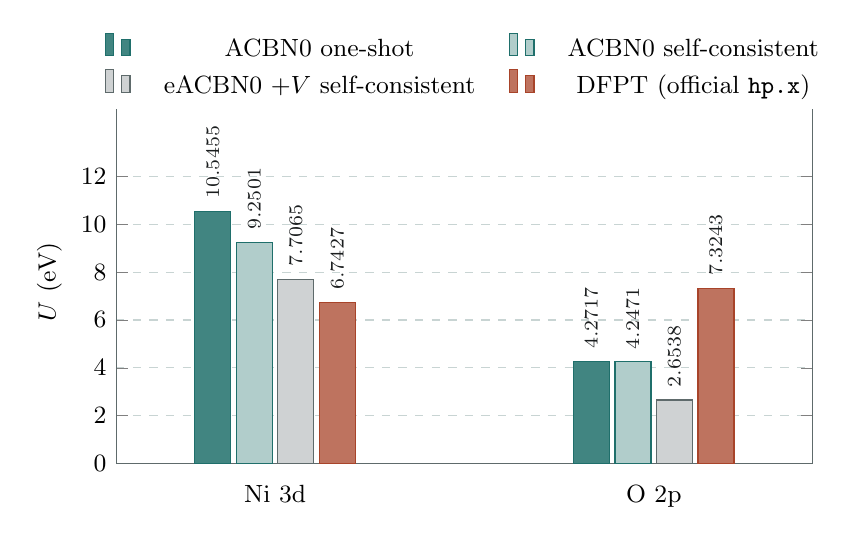
\begin{tikzpicture}
\begin{axis}[
  width=0.86\textwidth, height=6.2cm,
  ybar, bar width=13pt,
  enlarge x limits=0.42,
  ymin=0, ymax=15.2,
  ylabel={$U$ (eV)}, ylabel style={font=\small},
  ytick={0,2,4,6,8,10,12},
  symbolic x coords={Ni 3d, O 2p},
  xtick=data, xtick style={draw=none},
  tick label style={font=\small},
  ymajorgrids, grid style={rule,dashed,line width=0.4pt},
  axis line style={mute},
  legend style={at={(0.5,1.20)},anchor=north,legend columns=2,draw=none,
                font=\small,column sep=10pt,row sep=1pt},
  nodes near coords,
  every node near coord/.append style={font=\scriptsize,color=ink,
     rotate=90,anchor=west,xshift=1pt,
     /pgf/number format/fixed,/pgf/number format/precision=4,
     /pgf/number format/zerofill},
]
\addplot[draw=accent,fill=accent!85]   coordinates {(Ni 3d,10.5455) (O 2p,4.2717)};
\addplot[draw=accent,fill=accent!35]   coordinates {(Ni 3d,9.2501)  (O 2p,4.2471)};
\addplot[draw=mute,fill=mute!30]       coordinates {(Ni 3d,7.7065)  (O 2p,2.6538)};
\addplot[draw=rust,fill=rust!75]       coordinates {(Ni 3d,6.7427)  (O 2p,7.3243)};
\legend{ACBN0 one-shot, ACBN0 self-consistent, eACBN0 $+V$ self-consistent, DFPT (official \texttt{hp.x})}
\end{axis}
\end{tikzpicture}
\end{center}

\noindent
They disagree in \emph{opposite directions} on the two species: ACBN0 puts more
$U$ on the transition metal and less on the oxygen, DFPT the reverse. That
divergence, obtainable now from a single ground state, is the result.

\begin{itemize}[leftmargin=1.3em,itemsep=2pt]
\item \textbf{Self-consistency.} One-shot on bare DFT gives Ni 10.5455; at the
      ACBN0 fixed point, 9.2501. O barely moves: $4.2717 \to 4.2471$.
\item \textbf{Turning on $V$} (3.0~\AA\ cutoff, self-consistent) drops the
      on-site values to Ni 7.7065 and O 2.6538. The same screening is now shared
      between $U$ and $V$.
\item \textbf{Cost}, against an existing ground state on 128 cores:
      \textbf{2.6 s} CPU for \C{acbn0 = 1}, \textbf{19.3 s} for \C{acbn0 = 2}.
\end{itemize}

\subsection{The inter-site table, from that same single run}

Once V3 put the +V branch on \C{ldaU}, it could be pointed at the same official
ground state. The on-site $U$ comes back at \textbf{10.5455} and
\textbf{4.2717} --- identical to the +U-only branch to all six figures, from a
different kernel. That is correct rather than coincidental: the on-site ratio
depends only on on-site occupations, so the cutoff cannot move it in a one-shot
evaluation; it enters only through self-consistency.

\begin{center}\small
\begin{tabular}{lrrl}
\toprule
Pair & $d$ (\AA) & $V$ (eV) & shell \\
\midrule
Ni--O  & 2.0603 & \textbf{3.1859} & octahedral nearest neighbour \\
\midrule
Ni--Ni & 2.9020 & 1.4359 / 1.4357 & second shell \\
O--O   & 2.9020 & 0.8741          & second shell \\
Ni--Ni & 2.9254 & 1.4242 / 1.4244 & second shell, rhombohedrally split \\
O--O   & 2.9254 & 0.8671          & second shell, rhombohedrally split \\
\bottomrule
\end{tabular}\\[2pt]
{\footnotesize\color{mute} 19 neighbour cells; the 2.9020/2.9254 splitting is the AFM-II rhombohedral distortion.}
\end{center}

% ================================================================
\section{Stage V4: background channels}\label{sec:v4}

Stages S3 and V3 bought their move onto \C{ldaU} at one price: \C{ldaU}'s
scalar \C{Hubbard_l(nt)} names a single channel, so every \C{ehub_l(m,nt)} in
the transplanted kernels was collapsed to \C{Hubbard_l(nt)+1} and a type with
two channels was refused outright. V4 removes that restriction.

\subsection{The information was already there}

\C{ldaU} does store the same manifold \C{ldaV} does --- it just stores the
\emph{projectors} in up to three blocks instead of contiguously. In
particular \C{init_hubbard} builds

\begin{center}\small
\begin{tabular}{lll}
\toprule
\C{ldaV} & \C{ldaU} & stage V4 \\
\midrule
\C{ehub_lm(nt)}   & \C{ldim_u(nt)}   & \C{lm(nt)} \\
\C{ehub_lm_max}   & \C{ldmx_tot}     & \C{lm_max} \\
\C{ehub_l(m,nt)}  & \C{ll(m,nt) + 1} & \C{lch(m,nt)} \\
\C{ofstv(na) + m} & three-way, below & \C{ofs(m,na)} \\
\bottomrule
\end{tabular}
\end{center}

\noindent
\C{ll(m,nt)} (\C{ldaU.f90:290--320}) labels the concatenated manifold in
\emph{the same order} \C{ldaV} uses --- \C{Hubbard_l}, then \C{Hubbard_l2},
then \C{Hubbard_l3}. So the only genuinely missing piece was the map from a
manifold index to a \C{wfcU} column, which \C{MODULE hp_acbn0_man} now
supplies, following \C{force_hub.f90:1060--1071} and \C{copy_U_wfc}:

\begin{lstlisting}
m <=   2*l+1        ->  offsetU(na)       + m
m <= 2*(l+l2+1)     ->  offsetU_back(na)  + m -   (2*l+1)
otherwise, backall  ->  offsetU_back1(na) + m - 2*(l+l2+1)
\end{lstlisting}

\noindent
The XML question was settled by the same criterion that found bugs~1--3:
\C{Hubbard_l2}, \C{Hubbard_l3}, \C{Hubbard_U2} and \C{backall} \emph{do}
round-trip (\C{qexsd_copy.f90:434--441}, called at
\C{pw_restart_new.f90:1322}), and \C{init_hubbard} is re-run on \C{hp.x}'s
read path. A background channel counts as active only when
\C{Hubbard_U2} $\neq 0$, so a \C{HUBBARD} card that wants one must give it a
nonzero value --- 0.0001~eV is enough, and ACBN0 never reads it.

\subsection{Restoring 225 indices without guessing}

Undoing the collapse means putting the right $m$ back at 261 sites. Rather
than do that by hand, the fork was used as an oracle: our routines and
\C{new_ns_v.f90} were aligned statement by statement, and wherever an aligned
fork line carried \C{ehub_l(mX,nt)} where ours carried \C{lch(nt)}, the index
was spliced back --- but \emph{only} when the type argument matched and the
occurrence counts agreed. 215 sites resolved that way; the 10 that did not
were exactly the sites where an intended edit had broken the alignment, and
were done by hand against the fork.

That check earned its keep immediately. One of the ten was

\begin{lstlisting}
IF ( ehub_l(m1,nt) == 1 .AND. ehub_l(m2,nt) == 1 ) THEN     ! fork
IF ( lch(nt) == 1 ) THEN                                    ! V3
\end{lstlisting}

\noindent
--- a tautology under one channel, which V3 had legitimately simplified, and
which is \emph{wrong} the moment $m_1$ and $m_2$ can sit in different
channels. An earlier version of the splicing script silently skipped that
line, because the pattern meant to protect assignments (\C{lch(nt) =})
also matched the comparison (\C{lch(nt) ==}).

\subsection{A self-inflicted bug, caught by its own guard}

\C{hp_acbn0_build_man} ends by asserting that every state in the manifold
landed on a real \C{wfcU} column. On the first run it fired everywhere. The
cause was that the blanket rewrite of \C{offsetU(X)+Y} into \C{ofs(Y,X)} had
also rewritten the module's \emph{own definition} of that map, into
\C{ofs(m,na) = ofs(m,na)}. Without the assertion this would not have crashed:
\C{ofs} would have stayed 0 and every projection would have silently read
\C{wfcU} column~0. It is the same failure mode as bugs~3 and~4, and the reason
the guard was written in the first place.

\subsection{Result}

\begin{center}\small
\begin{tabular}{lrl}
\toprule
GaAs, Ga on-site \C{[1,1,4,4]} cell \C{[0 0 0]} & value (eV) & \\
\midrule
$U[s,s]$ & 0.9709 & \multirow{3}{*}{identical to \C{pw.x} on \C{ldaV}} \\
$U[s,p]$ & 0.5808 & \\
$U[p,p]$ & 0.3441 & \\
\midrule
\multicolumn{3}{l}{\C{hp.x} vs \C{pw.x}, same ground state: \textbf{204 / 204 lines identical}}\\
\multicolumn{3}{l}{manifold reported as \C{sp}, \C{ldim_u} $=1+3=4$, cost 0.27 s CPU}\\
\bottomrule
\end{tabular}
\end{center}

\noindent
And every single-channel case is bit-for-bit what stage V3 produced --- NiO
and MnO parameters identical, MnO still 168/168 against the authors' output.

% ================================================================
\section{Usage}

\begin{lstlisting}
 &inputhp
   prefix      = 'NiO',
   outdir      = './outdir',
   acbn0       = 2,     ! 0 = DFPT (default) | 1 = ACBN0 U | 2 = eACBN0 U+V
   nn_distance = 3.0,   ! d_IJ in Angstrom, required for acbn0 = 2
 /
\end{lstlisting}

\noindent
\C{acbn0 > 0} evaluates the parameters from the ground state in \C{outdir},
writes \C{eACBN0_hub.dat}, and stops before the $q$-point loop. The kernels
\emph{also} print the same \C{V[atom i, atom j, ...]} tables that \C{pw.x}
prints, which is what makes every comparison in this report a plain \C{diff}.

\smallskip
\noindent
\textbf{Both branches now read official QE's \C{ldaU}}, so both want an
ortho-atomic \C{HUBBARD} card with one channel per type, and both run on
\emph{any} such ground state --- including the very one DFPT consumes. Neither
needs \C{lacbn0} any more.

\smallskip
\noindent
\C{nn_distance} is the inter-site cutoff $d_{IJ}$, required for \C{acbn0 = 2}
unless the run carries \C{lda_plus_v} (in which case \C{ehub_nn_distance} comes
from the XML). Because \C{hp.x} now owns the neighbour table,
\textbf{the cutoff can be swept without re-running \C{pw.x}} --- which the fork
cannot do.

\smallskip
\noindent
One note on the reference inputs: \C{example/MnO.acbn0.in} declares its manifold
through \C{ehub_l_choice} and carries no \C{HUBBARD} card, so under V3 it needs
one added --- same manifold, \C{U = 0.0001} eV, numerically nothing. With that
single addition it still reproduces the reference across all 168 lines
(\C{MnO_ref_v3/}).

% ================================================================
\section{Regression suite}

\begin{center}\small
\begin{tabular}{llll}
\toprule
Tag & Case & Checks & Result \\
\midrule
\multirow{2}{*}{\C{acbn0 = 1}}
 & \C{NiO_acbn0}     & self-consistent, vs \C{pw.x} & \good\ PASS \ (9.2501) \\
 & \C{NiO_dual}      & one-shot on the DFPT ground state & \good\ PASS \ (10.5455) \\
\midrule
\multirow{4}{*}{\C{acbn0 = 2}}
 & \C{NiO_acbn0_v}   & self-consistent +V, vs \C{pw.x} & \good\ PASS \ (7.7065) \\
 & \C{NiO_type2_nn0} & cross-kernel, $d_{IJ}=0$ & \good\ PASS \ (9.2501) \\
 & \C{NiO_dual_v}    & one-shot +V on the DFPT ground state & \good\ PASS \ (10.5455) \\
 & \C{MnO_ref_v3}    & authors' recipe on \C{ldaU} & \good\ PASS \ (5.2344) \\
\midrule
external & MnO & 168/168 vs \C{example/MnO.acbn0.out} & \good\ PASS \\
\midrule
V3 $\to$ V4 & 6 cases & parameters unchanged by V4 & \good\ PASS $\times 6$ \\
\midrule
\multirow{2}{*}{V4}
 & \C{GaAs_v4} & Ga 4s+4p / As 4s+4p vs \C{pw.x} & \good\ PASS \ (204/204) \\
 & \C{GaAs_v4} & block structure $U[s,s]$/$[s,p]$/$[p,p]$ & \good\ PASS \\
\bottomrule
\end{tabular}
\end{center}

\begin{center}
\textbf{\textcolor{accent}{15 passed, 0 failed}} \quad --- one binary, one \C{make}.
\end{center}

% ================================================================
\section{Open items}\label{sec:open}

\subsection*{GaAs still cannot be validated against the \emph{authors'} reference}

Theirs is noncollinear with spin--orbit --- which dispatches to
\C{new_ns_e0_nc_1}, a separate $\sim$2300-line kernel set that was not
transplanted --- and it uses PBEsol \C{nc-fr} pseudopotentials where we have PBE
\C{nc_sr}. Wrong functional \emph{and} wrong relativistic treatment: unreachable
by construction, not by omission. Our GaAs run therefore compares our
\C{pw.x} to our \C{hp.x} --- which is exactly what stage V4 needs it for
(\S\ref{sec:v4}), since the question there is whether \C{ldaU} bookkeeping
reproduces \C{ldaV} bookkeeping, not whether either matches a spin-orbit
calculation. Reaching their numbers needs \C{new_ns_e0_nc_1} transplanted too.

\subsection*{\texttt{remove_ehub_u} has no route into \texttt{hp.x}}

It is input-only and is not round-tripped through the XML. We omit the factors,
which is correct whenever the \C{pw.x} run used the default of 1 --- but any
calculation that masks a channel (as their GaAs does) will disagree. The fix is
one \C{\&INPUTHP} tag.

\subsection*{\texttt{nspin = 1} is rejected, correctly}

Not our limitation: \C{init_lda_plus_v} refuses it at \C{ldaV.f90:103}, and the
A0/HF assembly hard-codes \emph{both} spin slots --- \C{p\%O(m3,m1,2,na)} on an
array dimensioned \C{(...,nspin,...)} --- so \C{nspin = 1} would read past the
end silently. Use \C{nspin = 2} with \C{starting_magnetization = 0.0}.

% ================================================================
\section{Artefacts}

\begin{center}\small
\begin{tabularx}{\textwidth}{lX}
\toprule
\C{HP/src/eACBN0.f90} & the deliverable: 4234 lines, 2 modules, 22 subroutines, 1 function \\
modified & \C{hpcom.f90}, \C{hp_readin.f90}, \C{hp_bcast_input.f90},
           \C{hp_main.f90}, \C{hp_print_clock.f90}, \C{Makefile},
           \C{make.depend} \\
backups  & \C{eACBN0.f90.\{s1,s2,s3,v1,v2,v3\}bak},
           \C{hp_readin.f90.\{bak,v2bak,v3bak\}}, \C{hp_main.f90.bak} \\
log      & \C{logs/260901-eacbn0-hpx.txt} \ (full session log, 1027 lines) \\
runs     & \C{/gpfs/yjkang/examples/hp/}: \C{NiO}, \C{NiO_acbn0},
           \C{NiO_acbn0_v}, \C{NiO_dual}, \C{NiO_dual_v}, \C{NiO_ref1shot},
           \C{NiO_type2_nn0}, \C{MnO_ref}, \C{MnO_ref_v3}, \C{GaAs_smoke},
           \C{GaAs_v4}, \C{_final_check} \\
\bottomrule
\end{tabularx}
\end{center}

\vspace{6pt}
\noindent\textcolor{rule}{\rule{\textwidth}{0.8pt}}
\vspace{2pt}

\noindent\footnotesize\color{mute}
Built with \texttt{tectonic} 0.17.0 in the \texttt{tex} micromamba environment.
Web version with the same figures:
\url{https://claude.ai/code/artifact/c7998bb7-d39c-426b-8752-387f33cb43f5}

\end{document}
